\section{Looking for communities with Markov Clustering}
\label{mcl}

In the next sections we explain in details the implementation of the
different phases of MCL.

\subsection{Convergency loop}
This loop is repeated a number of times, until the convergence is reached or the maximum
number of loops is executed.
The convergency loop is composed of 3 phases:
\begin{enumerate}
\item Matrix Multiplication, in which the current stochastic matrix is multiplied by itself
\item Matrix Inflation, an operation used to fasten convergency and whose aim and implementation will be explained in the following
\item Matrix Convergence Checker, used to compare achieved values with the previous ones.
\end{enumerate}

Given the matrix $A$ of step $i$, matrix $A'$ output of step $i+1$ has reached the convergency
if the following holds:
$$
\forall i,j . |A_{i,j} - A'_{i,j}| < \epsilon
$$ 
where $\epsilon$ is a parameter of the computation.
In order to minimize occupied space, to fasten convergency and to avoid pathological
cases to lead to "false convergency" (i.e. if the Markov Chain represented by the
matrix is characterized by periodicity), we decided to avoid matrix power method 
and to make the convergency loop proced as the Fibonacci series, meaning
that at step $i$ the matrix calculated in the loop will be $A^{fib(i)}$.
In the following, we will explain in detail the various phases in this convergency
loop.

\subsection{Matrix multiplication}
The first phase of the loop is \textbf{Matrix Multiplication}. For this part, we followed different
approaches for the implementation as map-reduce computations. While the first two approaches
revealed themselves to be very effective when dealing with dummy data using for the tests,
when real data was fetched both showed significant drawbacks that induced us to search for
a third solution, that is the one actually implemented in the delivered project.

Several implementations needed to be developed and tested in order to
achieve feasibility (onto the given environment) and improve performances.

\subsubsection{One step map-reduce}
In the beginning, we started by thinking that a simple approach could be producing all
couples to be multiplied of the two matrices with an appropriate index.\footnote{This algorithm
has been readapted and implemented starting from this website: http://importantfish.com/one-step-matrix-multiplication-with-hadoop/}
In this case, we have two different Map functions for two different files. To implement this in Map-Reduce, we exploited
the MultipleInputs function provided by the framework indicating for the two matrices a different mapper able
to emit different values.
The "first" matrix is fetched to the \texttt{OneStepRowMap} of fig. \ref{fig:onestepMaps} while the second to the \texttt{ColumnMap} of the same figure. In the pseudocode, there's no consideration for cases in which the value is 0, since the
matrix is already memorized neglecting null values.
The output of both mappers is fetched to \texttt{OneStepReduce} of fig. \ref{fig:onestepReduce}.
\begin{figure}[H]
\begin{verbatim}
//For both, value is a matrix entry, where (value.row,value.column) are the
//coordinates while value.probability is the actual value.
OneStepRowMap(key, value):
    for k = 1 to N:
        emit((value.row, k), ('A', value.column, value.probability))
OneStepColumnMap(key, value)
    for k = 1 to N:
        emit((k, value.column), ('B', value.row, value.probability))
\end{verbatim}
\caption{RowMap and ColumnMap used in the One-Step matrix multiplication algorithm. N is the size of the matrix, which is assumed to be square.}
\label{fig:onestep}
\end{figure}

\begin{figure}[H]
\begin{verbatim}
OneStepReduce(key, values):
//key is the coordinate of the element whose value is being calculated
//value is 'A' or 'B' (to distinguish between rows and columns), 
//row/column coordinate and probability
    A[N] = {j: a_ij for (x, j, a_ij) in values if x == A}
    B[N] = {j: b_jk for (x, j, b_jk) in values if x == B}
    result = 0
    for j = 1 to N:
        result += hash_A[j] * hash_B[j]
    emit(key, result)
\end{verbatim}
\caption{OneStepReduce used in the One-Step matrix multiplication algorithm. The key represents a single element in the matrix}
\label{fig:onestepReduce}
\end{figure}
As it is possible to understand, when dealing with actual data this kind of implementation could not
work, since for every matrix element $N=10^4$ elements are emitted. 
Elements are themselves $10^8$, making the total number of couples emitted by the mapper $10^{12}$.

Approximating the couple (key, value) with the size of its biggest component-
the double precision floating point probability values taking 128 bits on 64 word
machines - we would have needed a total memory of 128TB, which is much larger than
our enviroment total memory space, making impossible to carry on the computation
for dense matrices.

This implementation produced on our test environment a runtime exception caused by the termination
of spare secondary memory when the spills (after the map) were produced.

\subsubsection{Two step map-reduce}
The second approach has been the one of decomposing the computation further, trying to avoid
the explosion of data emitted caused by the algorithm discussed before.

In this approach, we have two map reduce steps.\footnote{Once again, this algorithmhas been readapted and implemented
following the post available at http://importantfish.com/two-step-matrix-multiplication-with-hadoop/}

In the mappers shown in fig. \ref{fig:twoStep1Map} used in the first step - again we distinguished between the two matrices using MultipleInputs - rows and columns values are emitted using their index as key.
In the reducer in fig. \ref{fig:twoStep1Reducer}the values of the row and column received are distinguished using the "A" and "B" flags. Subsequently,
every row value is multiplied for every column value, and this multiplied values are emitted using as key
the position of the value of the output matrix to which they will contribute. %todo: cec improbabol inglisc
\begin{figure}[H]
\begin{verbatim}
//For both, value is a matrix entry, where (value.row,value.column) are the
//coordinates while value.probability is the actual value.
TwoStepRowMap(key, value):
    emit(value.row, ("A", value.column, value.probability))

TwoStepColumnMap(key, value):
    emit(value.column, ("B", value.row, value.probability))
\end{verbatim}
\caption{Mappers used in the first phase of the two-step matrix multiplication algorithm.}
\label{fig:twoStep1Map}
\end{figure}
\begin{figure}[H]
\begin{verbatim}
TwoStepFirstReduce(key, values):
    //key is the index of the row/column
    //value is a flag "A" or "B" to distinguish between the two cases,
    //concatenated with the other coordinate (used in the list_*) and the value. 
    list_A = {(i, a_ij) for (M, i, a_ij) in values if M == "A"}
    list_B = {(k, b_jk) for (M, k, b_jk) in values if M == "B"}
    for (i, a_ij) in list_A:
        for (k, b_jk) in list_B:
            emit((i, k), a_ij*b_jk)
\end{verbatim}
\caption{Reducer used in the first phase of the two-step matrix multiplication algorithm.}
\label{fig:twoStep1Reducer}
\end{figure}

The second map-reduce phase of this algorithm implements the identity function in the mapper, and sums up all
multiplicated values for a certain value of the final matrix in the reducer shown in fig. \ref{fig:twoStep2Reducer}

\begin{figure}[H]
\begin{verbatim}
TwoStepSecondReduce(key, values):
//key is the coordinate of the element being calculated
//values is the list of the partial row by column products
    result = 0
    for value in values:
        result += value
    emit(key, result)
\end{verbatim}
\caption{Reducer used in the second phase of the two-step matrix multiplication algorithm, summing up al row-by-column values concurring in its calculation.}
\label{fig:twoStep2Reducer}
\end{figure}
Even though this algorithm is way more optimized with respect to the previous one, since it also avoids to emit intermediate couples for possibly null values, it has revealed to be very slow in practice. This is due, in our opinion, to the need
of writing intermediate data between the two steps of the job in HDFS, which slows down computation significantly.

Also in this case some disk problems could arise, because once again, in the worst case, the intermediate data between the two steps is in general $1/2$ of the one emitted by the mapper in the previous case, thus reproducing the usual disk issues for the data we were dealing with.
We will se how we solved this problem, by decomposing in smaller parts the input matrix, in the following part.

\subsubsection{Block-wise}
With this approach, to cope with the problems related to the disk, we divided the matrix into several blocks.
Blocks have been enforced to have always the same size, and the approach discussed below has been used.

Let $\mathbf{A}$ and $\mathbf{B}$ be two NxN matrix, and let $p$ be the number of row/column partitions given
as input parameter, meaning that $p^2$ blocks will be produced for each matrix. As an example, we can decompose
A as follows:
$$
\mathbf{A} =
\begin{bmatrix}
    \mathbf{A_{1,1}} & \mathbf{A_{1,2}} & ... & \mathbf{A_{1,p}} \\
    \mathbf{A_{2,1}} & ... & ... \\
    ... \\
    \mathbf{A_{p,1}} & ... & ... & \mathbf{A_{p,p}}
\end{bmatrix}
$$
Now let both $\mathbf{A}$ and $\mathbf{B}$ be decomposed as explained before, we can calculate a single block $\mathbf{C_{i,j}}$
of the matrix $\mathbf{C} = \mathbf{A} x \mathbf{B}$ as follows:
$$
    \mathbf{C_{i,j}} = \sum_{k=1}^{p} \mathbf{A_{i,k}} \times \mathbf{B_{k, j}}
$$
This approach allows, with a sufficient decomposition, to prevent any problem related to disk usage and, in the meanwhile,
produced with some test matrices a way faster computation in the latest implementation.
In fact, the inner multiplication - to be clear, the one between two blocks in the decomposition of the matrices given
as input of this phase - has been implemented in three different way:
\begin{enumerate}
\item In the first case, we tried the (now promising) one-step matrix multiplication algorithm proposed above. However also in this case the output of the mapper revealed himself as huge, as also for a $1/10$-th partition of the matrix (with 1000 values) this approach would produce $10^9$ values, which is certainly a manageable size but still big enough to make the I/O bottleneck significant and slow down the computation, specially when considering the huge number of such multiplications to perform to calculate the whole $\mathbf{C}.$
\item In the second case, to be honest merely impkemented for the sake of completeness, we tried also to plug-in as multiplication module the two-step matrix multiplication algorithm. As it could have been foreseen, also this approach - though faster than the previous one - was still not fast enough to meet our requirements.
\item The third case, which is the one used in the final project, revealed himself to be the best both in terms of space and in completion time. This algorithm merely multiplies two blocks using the good old $O(n^3)$ sequential row-by-column matrix multiplication.
\end{enumerate}

The approach that we finally decided to follow is very efficient for several resons.
Consider the case in which the number of partitions is 10, thus achieving 100 blocks for each of the two multiplied matrices.
The blocks will contain, in a worst case approximaton, $10^6$ doubles, meaning that a block multiplication will fit in memory and thus result in better performances, since also the output of each block-by-block multiplication will have size of approximately 32MB each, considering also the indexes.

Notice that this values, on our environment, allow to multiply several blocks in parallel, leading to a very good utilization
factor of the machines and nice results in terms of completion time.
The detailed implementation of this part is discussed thoroughly in \ref{blockmul}.

\subsubsection{Block-wise multiplication implementation}
\label{blockmul}
We wanted to develop, in this part, an highly parametrized system so to finely tune our computation to make it faster,
given that this is the biggest contributor to the completion time of the convergency loop, which is executed also several times.
For this reason, a module, called BlockWiseMatrixMultiplication has been developed, with the aim of allowing parametrized execution.

This module, which implements the \texttt{Tool} interface of the Hadoop framework, can be executed specifying the number
of blocks of the final matrix $\mathbf{C_{i,j}}$ to be calculated in parallel. It takes also in input the directory containing
the two input matrices splitted in blocks and the directory in which the results must be written. 
Partitions are calculated automatically scanning the blocks by horizontal coordinates (by row) and then by column.

For each block multiplication scheduled by this very simple partitioner, a new thread is forked, which is responsible
for starting and monitoring all the jobs (running in parallel) consisting of the multiplications $\mathbf{A_{i,k}} \times \mathbf{B_{k,j}}$ needed to calculate $\mathbf{C_{i,j}}$.

In order for them to run in parallel, we used the \texttt{JobControl} class of the Hadoop framework, which allows to
schedule parallel jobs (and also to define dependencies between jobs). For every output block $\mathbf{C_{i,j}}$ $p$ 
multiplications of the original matrix blocks are performed as independent jobs running in parallel. 
These jobs consist of a single map-reduce phase, in which the mappers (as usual, one for the row and one for the column exploiting MultipleInputs) of fig. \ref{fig:blockwisemap} take care of "joining" and labelling the two blocks to be multiplied.
In the reducer, the whole blocks are gathered and saved in a matrix, which is then multiplied before the final values
are written in output, as it is possible to see in fig. \ref{fig:blockwisereduce}.
In the reducer, a slight optimization has been achieved by memorizing the second matrix (accessed $N/p$ times) by column
and not by row, to avoid jumps in memory and to exploit caches in the best possible way.

\begin{figure}[H]
\begin{verbatim}
//for both, value is a block element, with form value.blockHorizontalIndex,
//value.BlockVerticalIndex, value.row_id, value.column_id, value.probability
BlockRowMapper(key, value):
    emit(
      value.blockVerticalIndex, 
      ('A',value.row_id,value.column_id, value.probability)
    )

BlockColumnMapper(key, value):
    emit(
       value.blockHorizontalIndex,
       ('B', value.row_id, value.column_id, value.probability)
    )
\end{verbatim}
\caption{Mappers used in the block-wise matrix multiplication. The block $\mathbf{A_{i,k}}$ is managed by BlockRowMapper, while $\mathbf{B_{k,j}}$ by BlockColumnMapper. This names are given merely for consinstency wrt. previous algorithms. Notice that row\_id and column\_id are coordinates local to the block.} 
\label{fig:blockwisemap}
\end{figure}

\begin{figure}[H]
\begin{verbatim}
//key is k, to merge Aik and Bkj
//values is the list of elements belonging to the two blocks, 
//each one comprising a label (A, B)to distinguish between the 
//two blocks, the local coordinates and the probability 
MatrixMultiplicationReducer(key, values):
    A[N/p][N/p]
    B[N/p][N/p]
    for v in values
        if v.label = 'A'
            A[v.row_id][v.col_id] = v.probability
        else
            B[v.col_id][v.row_id] = v.probability
    for i in [1, N/p]
        for j in [1, N/p]
            sum = 0
            for k in [1, N/p]
                sum += A[i][k]*B[j][k]
            if sum > 0
                emit((i,j), sum)
\end{verbatim}
\caption{Reducer used in the block-wise matrix multiplication. It performs the usual row-by-column matrix multiplication algorithm. N is the size of the matrix, p is the number of splits}
\label{fig:blockwisereduce}
\end{figure}
The second job needed to finally compute $\mathbf{C_{i,j}}$ is the one performing the sum over all partial matrices produced before, in order to achieve the real values of the computed block.
This job has, in its configuration, the horizontal and vertical coordinates $i$ and $j$ of the output block. In its mapper of fig. \ref{fig:blocksummap}, it aggregates by block row id and block column id the elements, so that they can be subsequently summed in the reducer as of fig. \ref{fig:blocksumreduce}.
This job is dependant of the previous ones, thus starts as soon as all the input data needed has been produced.
\begin{figure}[H]
\begin{verbatim}
//value is a block element, with local row_id, local column_id and probability 
BlockSumMapper(key, value):
    emit((value.row_id, value.col_id), value.probability)
\end{verbatim}
\caption{The map function used to perform the sum over all partial matrices $\mathbf{A_{i,k}} \times \mathbf{B_{k,j}}$ and thus to calculate $\mathbf{C_{i,j}}$}
\label{fig:blocksummap}
\end{figure}
\begin{figure}[H]
\begin{verbatim}
//Takes as context parameter the coordinates of the block currently calculated
//key is the local coordinate within the block
//values is the list of probabilities to be summed
BlockSumReducer(key, values):
    blockIdX = context.horizontal_coordinates
    blockIdY = context.vertical_coordinates
    sum = 0
    for v in values
        sum += v
    emit((blockIdX, blockIdY, key.row_id, key._column_id), sum)
\end{verbatim}
\caption{The reduce function used to calculate the sum over single values in a position of the block and which writes out the final block.}
\label{fig:blocksumreduce}
\end{figure}
The thread forked and running the JobControl containing all such "individual block" jobs running in parallel, is checked periodically by another thread for completion. When this phase terminates, another set of blocks of parametric size
is calculated and the related multiplications are run.
This approach of not running everything in parallel has been pursued in order to avoid disk space issues and also to be 
able to avoid too much contention in the system.
From experimental results, in fact, we were able to verify that the matrix multiplication can be made very fast by dividing
initial matrices in 25 blocks and using partitions of size from 5 (corresponding thus to an entire row).

The drawback of this approach is that some others modules - for decomposing and recomposing the matrix - must be executed, as we wanted our procedure not to affect the final matrix representation.
These modules implementation is discussed in \ref{splitter} and \ref{recombiner}.
Finally, the behaviour of a single block multiplication is sketched in fig. \ref{fig:blockmultiplicationsketch}, while
the comprehensive driver of the matrix multiplication procedure that we finally adopted is illustrated in fig. \ref{fig:matrixmultiplicationsketch}, and its source code can be seen on %todo: insert link.

\begin{figure}[H]
\centering
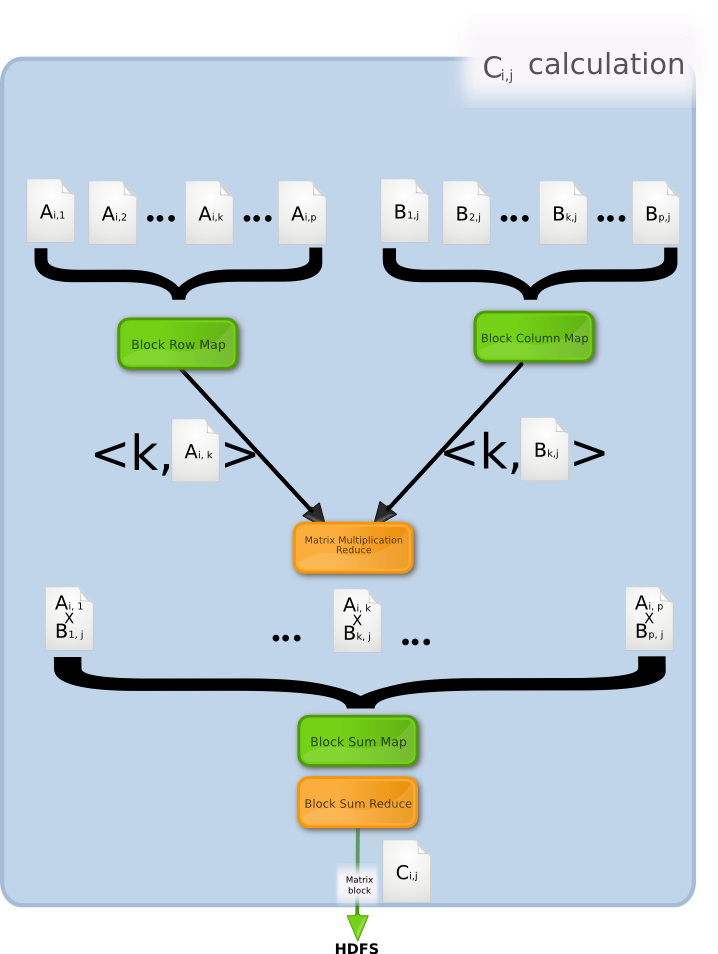
\includegraphics[scale=0.7]{blockmultiplication.png}
\caption{Procedure followed to calculate a single $\mathbf{C_{i,j}}$.}
\label{fig:blockmultiplicationsketch}
\end{figure}

\begin{figure}[H]
\centering
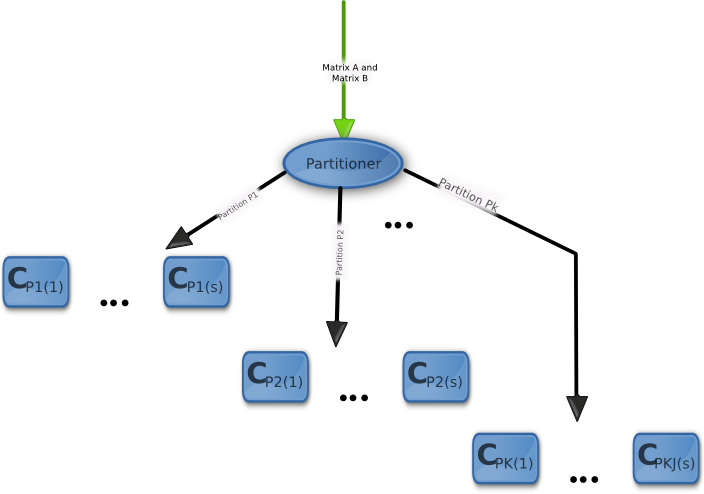
\includegraphics[scale=0.7]{matrixmultiplication.png}
\caption{Whole matrix multiplication procedure in a block-wise fashion. S blocks of the matrix are calculated
in parallel, while the others wait for the completion of the previous ones before going on.
In the image, s is the maximum size of the partition, k is assumed as the number of partitions and Pi(n) is a function
returning the index of the n-th block in partition Pi.In the image, the blue blocks titled after the matrix block they are used to compute represent the calculation shown in fig. \ref{fig:blockmultiplicationsketch}}
\label{fig:matrixmultiplicationsketch}
\end{figure}

\subsection{Inflation}

After multiplying the matrix by the last precedently computed, we apply a strategy
called inflation in order to enlarge differences between elements in a row.
Using the algorithm author words: ''richests get richer, poorests get poorer''.
In fact our main purpose is to emphasize strong connections and to hide
weak ones.

For each row, we compute the sum of all r-th powers of its elements.
Then we recompute the element i,j as
$$ a_{i,j} = \frac{a_{ij}^r} {\sum_{k=0..N} a_{ik}^r}$$

Once again, this can be done in a single map reduce job. However, in the mapper as of fig. \ref{fig:inflationMap} we will need to recompose the rows, in order to gather them all together in the reducer. In this last phase whose pseudo-code is displayed in fig. \ref{fig:inflationReduce} re-scaled values will be divided once again in blocks.

\begin{figure}[H]
\begin{verbatim}
//value is a matrix block record in the form block_horizontal_id, block_vertical_id
//row_id, column_id, probability.
InflationMap(key, value):
   col = value.block_vertical_id * (N/p) + value.column_id
   row = value.block_horizontal_id * (N/p) + value.row_id
   emit(row, (col, value.probability))
\end{verbatim}
\caption{Pseudo code for the mapper used in the Inflation phase. Since the procedure requires a rescaling of all values depending
on the sum of the power of the values in a certain row, the original row must be recomposed from the blocks. 
We remember that N is the size of the matrix, while p is the number of splits and they are both parameters for this computation.}
\label{fig:inflationMap}
\end{figure}

\begin{figure}[H]
\begin{verbatim}
//key is the absolute row coordinate
//value is a couple with absoulte column coordinate and actual probability
//r is the inflation parameter, passed along with the context
InflationReduce(key, values):
    row_list = []
    r = context.inflationParameter
    sum = 0
    for v in values:
        curV = v.probability^r
        sum += curV
        row_list.add((v.column, curV))
    if sum == 0: return
    splitSize = N/p
    blockX = floor(key/splitSize)
    localRow = key % splitSize
    for v in row_list:
        blockY =  floor(v.column / splitSize)
        localCol = floor(v.column % splitSize)
        inflatedV = v.probability / sum
        emit(
            (blockX, blockY, localRow, localCol),
            inflatedV
        )
\end{verbatim}
\caption{}
\label{fig:inflationReduce}
\end{figure}

\subsection{Convergency}
The convergency checker is a simple map-reduce job. The mapper takes as input two matrices, the one 
newly calculated and the one calculated in the previous step. 
Then, as shown in fig. \ref{fig:convergencyMap} , it emits the probability for a certain value using as key its coordinates, which
in this case are represented by two couples, the former referring to the block and the latter to the
relative position inside the block.
\begin{figure}[H]
\begin{verbatim}
//value is block_horizontal_id,block_vertical_id \t row_id, col_id \t probability
//for the previous and current matrix
ConvergenceMap(key, value):
    emit(
       (value.block_horizontal_id,
        value.block_vertical_id,
        value.row_id,
        value.col_id
       ),
       value.probability
    )
\end{verbatim}
\caption{Pseudo code of the mapper used to implement the convergency. This mapper aggregates values of the current and previous matrix
by their coordinate; their value will then be compared in the reducer.}
\label{fig:convergencyMap}
\end{figure}

In the reducer shown in fig. \ref{figure:convergencyReduce}, these two values are subtracted and their difference confronted against the threshold. Whenever the difference is bigger than the threshold, a \texttt{Counter}, provided by the Hadoop framework is incremented by one,
making the job (whose output is always empty) return the number of non converged values.
The threshold is a parameter of the computation, which is by default set to $0.0001$.

\begin{figure}[H]
\begin{verbatim}
//values is a couple of values coming from the previous and the current matrix. 
//context has a counter used to take note of the number of non converged values and
//a threshold, which is a parameter set by default to 0.0001
ConvergenceReduce(key, values):
   p1 = value[1] or 0
   p2 = value[2] or 0
   if abs(p1-p2) > context.threshold:
      context.counter++; 
\end{verbatim}
\caption{Pseudo code of the reducer used to check for the convergency. The \texttt{threshold} is a parameter of the computation. The counter is a feature provided by the Hadoop framework}
\label{figure:convergencyReduce}
\end{figure}

Finally the driver checks for the value of this counter as soon as the job finishes, to check if a new convergency iteration
has to be executed or if the matrix has converged.
To better understand the convergency speed of our algorithm, we kept track of the number of non converged values during the
execution of Markov Clustering. 
As we show in \ref{fig:convergencyGraph} we observed that in the beginning values tend to converge very fast, approximately halving at every iteration for the first 6-7 iterations. Thereafter, the number of non-converging values continues to decrease
but in a more slow fashion, arriving from 16th iteration on to decrease only of an order of 10 values for iteration, and in some cases even to stop. However, it is possible to observe that the number of non-converged values after 10 iterations is in general very small, usually about 2000 and thus represents only the 0.2\% of the total values.
\begin{figure}[H]
\centering
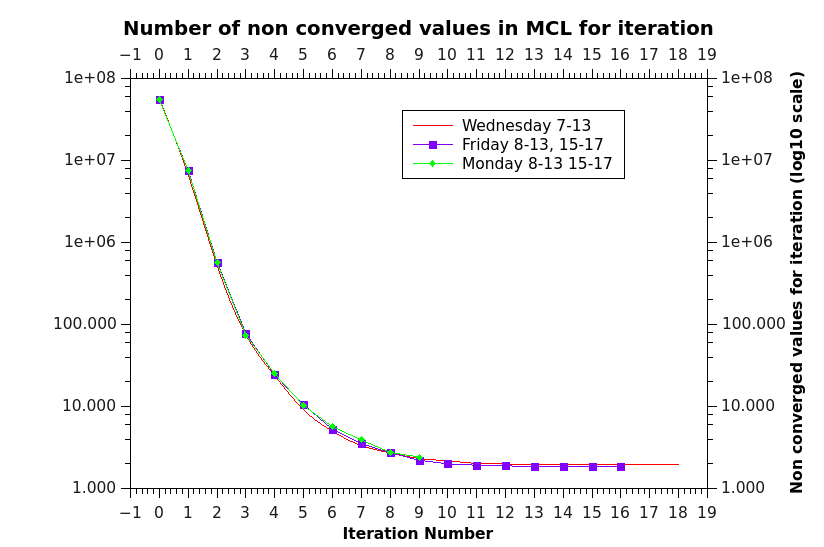
\includegraphics[scale=0.8]{convergency.png}
\caption{Number of non converged values for every iteration. The number of values is in logarithmic scale. We can see that, while in the beginning the number of non converged values is in the order of the matrix size, this number very rapidly decreases as the clustering iterations proceeds, to finally stabilize around 2000 from 10th iteration on.}
\label{fig:convergencyGraph}
\end{figure}
When we noticed this behaviour, we decided to switch from a 20-iteration clustering to a 10 iteration one. The idea is that, even though the number of non converged values will in general be higher than in the 20 iteration case, we prefer to have a faster computation even at the cost of precision, since further iterations won't significantly affect the quality of the clusters.

\subsection{Matrix splitter}
\label{splitter}
The execution of this map reduce job occurs twice in a whole MCL execution, and as previously said it is needed in order to
perform a blockwise multiplication.
In the beginning, when the average probability graph is fetched to the clustering procedure, the matrix representing it must be
divided into blocks.
During the map execution of this block, starting from the global coordinates of each matrix element, the block horizontal
and vertical identifier are calculated, as well as the row and column of every element inside the corresponding block.
This can be seen in \ref{fig:splitterMap}

\begin{figure}[H]
\begin{verbatim}
//value is a matrix element, with row, column and probability
SplitterMap(key, value):
	splitSize = N/p
    blockX = floor(value.row/splitSize)
    localRow = value.row % splitSize
    blockY = floor(value.column/splitSize)
    localCol = value.column % splitSize
    emit(
        (blockX, blockY),
        (localRow,localColumn,value.probability)
    )
\end{verbatim}
\caption{Mapper used in the matrix splitting procedure. Remember that N is the size of the matrix and p is the size of the split, passed to the actual map tasks through the context.}
\label{fig:splitterMap}
\end{figure}
The reducer of fig. \ref{fig:splitterReduce} takes the newly calculated coordinates grouping the values by the block to which they belong.
Then, exploiting the \texttt{MultipleOutput} function of the Hadoop framework, a new file is generated for each block. The destination file
to which the values and their coordinates will be written will be function of the block coordinates evaluated in the previous step.

\begin{figure}[H]
\begin{verbatim}
//key is the coordinate of the block to which the value belong
//value is composed by local row and column id and by the value.
SplitterReduce(jey, values)
	for v in values:
		emit(key, v) on file(key)
\end{verbatim}
\caption{Reducer used in the matrix splitting procedure. This reducer uses MultipleOutputs in order to write different blocks on different folders (represented by \texttt{file(key)} in the pseudocode), allowing to operate seamlessly in parallel on several blocks in the consecutive steps.}
\label{fig:splitterReduce}
\end{figure}

\subsection{Matrix recombiner}
\label{recombiner}
The matrix recombiner is the final step of our work to be performed using map-reduce. To be more precise, this job is composed only
by a map, while there's no reduce phase. The aim of this part of our work is to gather all the blocks of the latest calculated matrix and recompose all values with global coordinates under a unique folder, preparing for the execution of the next phase, described in \ref{findingcluster}. 
The pseudo-code of such mapper (which is kind of obvious) can be seen in fig. \ref{fig:recombiner}
\begin{figure}[H]
\begin{verbatim}
//value is block_horizontal_id, block_vertical_id, row_id, column_id, probability
RecombinerMap(key, value):
    splitSize = N/p;
    absoluteRow = value.block_horizontal_id*splitSize+value.row_id
    absoluteCol = value.block_vertical_id*splitSize+value.column_id
    emit((absoluteRow, absoluteCol), value.probability)
\end{verbatim}
\caption{Matrix recombiner map. We remember that N is the size of the matrix and p is the number of partitions for every dimension of the matrix.}
\label{fig:recombiner}
\end{figure}

\subsection{Driver}
The driver for the Markov Clustering algorithm that we implemented is thus composed of several phases.
It takes as input parameters the following values:
\begin{enumerate}
\item \textbf{Input folder}, containing a probability matrix to be seen as a Markov Chain
\item \textbf{Output folder}, where the results will be written
\item \textbf{Maximum number of iterations}, the maximum number of convergency loops to perform before stopping
\item \textbf{Number of workers}, parameter used to decide how many matrix blocks multiplications should be computed in parallel.
\end{enumerate}
Starting from this phase, in the beginning the matrix is pre-processed and divided in blocks. The matrix is replicated on two different directories, that will be fetched in input to the first matrix multiplication phase.

The matrix multiplication phase works operating on 3 directories. It rotates in modulo 3 wrt to iteration number, taking the first two as input and the last as output folder.
However, the matrix multiplication writes on a temporary "inflate" directory. It will be the Inflation module responsible for filling the output dir of the phase with the ultimate result.
The convergency phase, instead, as previously explained, doesn't write down any information on the disk but merely exploits hadoop counters to understand the number of non converged values existing in the matrix.
Finally, when the matrix converges or the number of maximum iterations has been reached, the matrix is recomposed and written in the output directory.

A sketch depicting the behaviour of the whole pipeline that we developed can be seen in fig. \ref{fig:completepipeline}
\newpage
\begin{figure}[H]
\centering
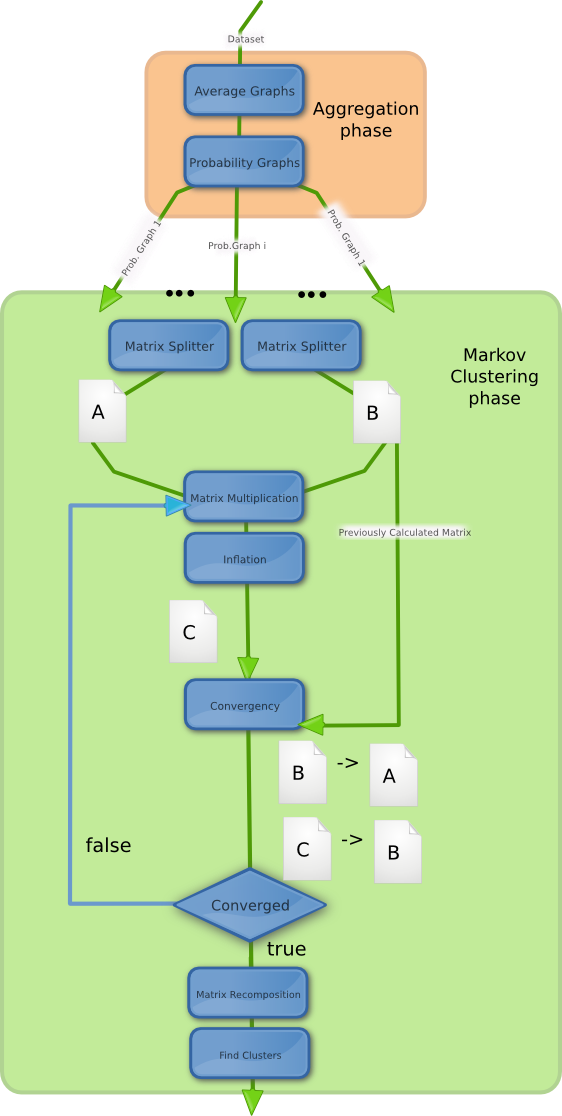
\includegraphics[scale=0.7]{completepipeline.png}
\caption{Pipeline of the computation}
\label{fig:completepipeline}
\end{figure}
\newpage
\subsection{Finding clusters}
\label{findingcluster}
By the definition given in the original paper, given a matrix
multiplied until convergency is reached, the clusters are
identified as disjoint components in the graph, that means
a partition of the set of nodes such that there are no edges
linking two nodes which belong two different subsets in the partition.

In the  final matrix actually, values that are not 0 are 1 or tend to 1
and since this is stochastic matrix, this means that for each row
only one value is different from zero.

This, in turn, means that our aim of reduce the graph density toward
a linear number of edges, w.r.t the number of nodes, were  actually reached.

In this scenario, it is much more probable to discover disjoint compoments
of the graph, i.e clusters, i.e communities.

We implemented the last module of our application, the DisjointComponentVisit
class, as a visit
of the graph able of recognizing the different disjoint componets, which
defines and uses three main actions:
\begin{itemize}
    \item \verb!new_component()! creates a new subset of nodes,
    \item \verb!merge_components(c1,c2)! merges two subsets into one,
    \item \verb!add_to(n,c)! add a node to a subset.
\end{itemize}

The module, cycles over all edges in the result files, looks
for the components containing the head and the tail of the egde,
the in case they are the same it continues. If the head and tail
belong to different component, they are merged into one.
If one of the two nodes does not belong to any components, it is
added  to the component of the other one (in case none of them 
are contained in any components, a new component is created and both
are added to it).

We used the Java class \verb!java.util.TreeSet! to implement
the components which assures logarithmic time for
the operations of adding a new element and testing if an element
is contained. 

Since the expected result of convergency is that all non-zero edges
are one, dunring this visit edges with weight values less than $0.9$
are discarded. This is due becase of the approximention done by
posing a maximum number of iterations to the convergency loop.

After all components are computed, we generate three files:
\begin{itemize}
\item a text file called \verb!clusters.txt! with all the components and
the list of the nodes within it,
\item a PNG file called \verb!clusters.png! displaying all the edges and
\item a PNG file called \verb!patchwork.png! displaying the grid where
each node is coloured with a different color depending on the cluster it
is in.
\end{itemize}


